\documentclass{beamer}
\usepackage{amsmath}
\usepackage{circuitikz}
\usepackage{tikz}
\usetheme{CambridgeUS}
\usepackage{tcolorbox}
\title{Electricity and Magnetism}
\author{Birendra Bdr. Dhanuk}
\institute{Namuna Secondary School Ladavir}
\date{\today}

\begin{document}

%The next statement creates the title page.


\frame{\titlepage}

\begin{frame}
\frametitle{Contents:}
\tableofcontents
\end{frame}

% Slide for Chapter: Electrical Circuits
\section{Electrical Circuits}

\begin{frame}
\textcolor{green}{Kirchhoff's law }\\
Kirchhoff's laws are fundamental in circuit analysis, consisting of two rules: the Kirchhoff's Current Law (KCL) and the Kirchhoff's Voltage Law (KVL).

\textcolor{red}{1. Kirchhoff's Current Law (KCL)}

\textbf{Statement:} The total current entering a junction is equal to the total current leaving the junction. Mathematically,  
\[
\sum I_{\text{in}} = \sum I_{\text{out}}
\]

\textbf{Explanation:} At any junction in an electrical circuit, charge is conserved, so the sum of incoming currents equals the sum of outgoing currents.

\begin{center}
\begin{circuitikz}
\draw
  (0,0) node[below]{$I_1$} -- (1,1)
  (1,1) -- (2,2) node[above]{$I_2$}
  (1,1) -- (2,0) node[below]{$I_3$};
\draw[->] (0,0) -- (1,1);
\draw[->] (1,1) -- (2,2);
\draw[->] (1,1) -- (2,0);
\node at (1.5,1.4) {\(I_1 = I_2 + I_3\)};
\end{circuitikz}
\end{center}
\end{frame}

\begin{frame}

\textcolor{red}{2. Kirchhoff's Voltage Law (KVL)}

\textbf{Statement:} The sum of all voltages around a closed loop in a circuit is zero. Mathematically,  
\[
\sum V = 0
\]

\textbf{Explanation:} In any closed loop, the energy gained by charges from sources (like batteries) is equal to the energy lost through resistors or other components.

\begin{center}
\begin{circuitikz}
\draw
  (0,0) to[battery, v_=$V_1$] (0,3)
  to[resistor, l_=$R_1$, v_=$V_2$] (3,3)
  to[resistor, l_=$R_2$, v_=$V_3$] (3,0)
  -- (0,0);
\node at (4,2) {\(V_1 - V_2 - V_3 = 0\)};
\end{circuitikz}
\end{center}
\end{frame}

\begin{frame}
\textcolor{green}{\textbf{Wheatstone bridge Circuit}}


\textcolor{red}{Wheatstone Bridge}\\

The Wheatstone Bridge is an electrical circuit used to measure an unknown resistance by balancing two legs of a bridge circuit. It operates based on the principle of null deflection, where no current flows through the galvanometer when the bridge is balanced.\\

\textcolor{blue}{Circuit Diagram:}
\begin{center}
\includegraphics[width = 5 cm]{WheatstoneBridge}
\end{center}


\end{frame}

\begin{frame}


\textbf{Balance Condition:}
\[
\frac{R_1}{R_2} = \frac{R_3}{R_4}
\]
When the bridge is balanced, the ratio of resistances in one leg equals the ratio in the other leg, and no current flows through the galvanometer.

\vspace{0.5cm}

\textcolor{red}{Meter Bridge}\\

The Meter Bridge is a practical form of the Wheatstone Bridge used to measure unknown resistances. It consists of a one-meter-long wire of uniform cross-sectional area stretched over a meter scale.\\

\textcolor{blue}{Circuit Diagram:}
\begin{center}
\includegraphics[width = 5 cm]{meterbridge}
\end{center}
\end{frame}

\begin{frame}
\textbf{Working Principle:}  
The balance condition is achieved by adjusting the jockey on the wire until the galvanometer shows zero deflection. The unknown resistance \(R\) is then calculated using:
\[
\frac{R}{S} = \frac{l}{(100 - l)}
\]
where \(l\) is the balancing length.




\textcolor{green}{Potentiometer}

The potentiometer is an instrument used to measure the electromotive force (emf) of a cell, compare the emfs of two cells, and determine the internal resistance of a cell. It works on the principle that the potential difference across a uniform wire is directly proportional to its length when a constant current flows through it.

\textcolor{red}{1. Comparison of EMFs}

The potentiometer can be used to compare the emfs of two cells.

\end{frame}

\begin{frame}
\textcolor{blue}{Circuit Diagram:}
\begin{center}
\begin{circuitikz}
\draw
  (0,0) to[battery, l_=$E$] (0,3) 
  to[resistor, l_=$R$] (6,3)
  -- (6,0) -- (0,0);
\draw
  (2,3) -- (2,0) to[switch] (4,0) -- (4,3);
\draw
  (4,0) -- (5,-1.5) to[battery, l_=$E_1$] (3,-1.5) to[galvanometer] (2,-1.5) -- (4,0);
\draw
  (4,0) -- (7,-1.5) to[battery, l_=$E_2$] (5,-1.5);
\draw
  (4,3) -- (4.5,1.5) node[right] {Sliding Contact};
\node at (5,2.5) {\(L_1\)};
\node at (7,2.5) {\(L_2\)};
\end{circuitikz}
\end{center}

\textbf{Mathematical Formulation:}  
Let \(L_1\) and \(L_2\) be the balancing lengths for the two cells \(E_1\) and \(E_2\), respectively. Since the potentiometer works on the principle of a null deflection, we have:
\[
\frac{E_1}{E_2} = \frac{L_1}{L_2}
\]
\end{frame}


\begin{frame}
\textcolor{red}{2. Measurement of Internal Resistance of a Cell}

The potentiometer can also be used to measure the internal resistance \(r\) of a cell.

\textcolor{blue}{Circuit Diagram:}
\begin{center}
\begin{circuitikz}
\draw
  (0,0) to[battery, l_=$E$] (0,3) 
  to[resistor, l_=$R$] (6,3)
  -- (6,0) -- (0,0);
\draw
  (2,3) -- (2,0) to[ammeter] (4,0) to[switch] (4,3);
\draw
  (4,0) -- (5,-1.5) to[battery, l_=$E$] (3,-1.5) to[galvanometer] (2,-1.5) -- (4,0);
\draw
  (4,3) -- (4.5,1.5) node[right] {Sliding Contact};
\node at (5,2.5) {\(L_1\)};
\node at (7,2.5) {\(L_2\)};
\end{circuitikz}
\end{center}
 
1. Let \(L_1\) be the balancing length when the cell is in open circuit.  
2. Let \(L_2\) be the balancing length when the cell is connected to a known resistance \(R\).  
\end{frame}


\begin{frame}
The internal resistance \(r\) is given by:
\[
r = R \left(\frac{L_1}{L_2} - 1\right)
\]

\textbf{Explanation:}  
The balancing length \(L_1\) corresponds to the emf of the cell, while \(L_2\) corresponds to the potential difference across the cell when it delivers current through \(R\). The difference allows the calculation of \(r\).
\end{frame}

\begin{frame}
\textcolor{red}{Conversion of Galvanometer to ammeter}
\begin{center}
\includegraphics[width = 6 cm]{gtoam}
\end{center}

\begin{itemize}
\item \textbf{Galvanometer:} A galvanometer is a sensitive device used to detect small currents.
\item \textbf{Add Shunt Resistor:} Connect a low-resistance shunt resistor in parallel with the galvanometer.
\item \textbf{Low Resistance:} The shunt should have a very low resistance to allow most current to bypass the galvanometer.
\item \textbf{Current Range:} The total resistance determines the ammeter’s current range.
\item \textbf{Calibration:} Calibrate the scale to show current instead of voltage.
\item \textbf{Adjust Sensitivity:} Ensure the galvanometer can measure small currents accurately without damage.
\item Calculate the shunt resistance using the formula:
$R_s=\frac{I_g G}{I-I_g}$
\end{itemize}

\end{frame}

\begin{frame}
\textcolor{red}{Conversion of Galvanometer to voltmeter}
\begin{center}
\includegraphics[width = 6 cm]{gtov}
\end{center}
\begin{itemize}

\item \textbf{Add Shunt Resistor:} Connect a large resistor in series.
\item \textbf{High Resistance:} Ensure the shunt has high resistance.
\item \textbf{Calibrate:} Adjust for accurate voltage readings.
\item \textbf{Voltage Range:} Set the total resistance for desired range.
\item \textbf{Adjust Scale:} Modify the scale to read voltage.

The voltage across the galvanometer at full-scale deflection is:

\[
V_g = I_g \cdot G
\]

To measure the maximum voltage \( V_{\text{max}} \), the total resistance of the voltmeter should be:

\[
R_{\text{total}} = \frac{V_{\text{max}}}{I_g}
\]


\end{itemize}

\end{frame}



\begin{frame}
Now, the multiplier resistance \( R_m \) is the difference between the total resistance and the resistance of the galvanometer:

\[
R_m = R_{\text{total}} - G = \frac{V_{\text{max}}}{I_g} - G
\]

Thus, the multiplier resistance required to convert the galvanometer into a voltmeter is:

\[
R_m = \frac{V_{\text{max}}}{I_g} - G
\]
\end{frame}



\begin{frame}
\textcolor{red}{\textbf{Joule's Law of Heating}}\\
According to this law, the amount of heat (H) developed in an ohmic conductor by the passage of current I .\\
\begin{itemize}
\item[1] Directly proprtional to the square of the current $i.e. H\propto I^2$
\item[2] Directly proportional to the resistance of the conductor $H\propto R$
\item[3] Directly proportiona to the time flow of current $H\propto t$
\end{itemize}
On Combining above reltion we get,\\
\hspace{2cm} $H\propto I^2Rt$\\
\hspace{2cm} $H=kI^2Rt$\\
Where, k is the proportionality constant. The value of k depends on the system of unit of heat.\\
$k=\frac{1}{j}$ is the unit conversion factor. and Its value is 4.2 J/calorie.
\end{frame}





\begin{frame}
\begin{tcolorbox}[colback=green!10!white, colframe=green!50!black, title=Verification of Joule's Law]
To verify Joule's Law experimentally, we focus on the following three points:

\begin{enumerate}
    \item \textbf{Heat is directly proportional to the square of the current (\( I^2 \)):} \\
    By varying the current and keeping \( R \) and \( t \) constant, measure the heat produced. A plot of \( H \) vs \( I^2 \) should yield a straight line.

    \item \textbf{Heat is directly proportional to the resistance (\( R \)):} \\
    By varying the resistance and keeping \( I \) and \( t \) constant, measure the heat produced. A plot of \( H \) vs \( R \) should yield a straight line.

    \item \textbf{Heat is directly proportional to the time (\( t \)):} \\
    By varying the time and keeping \( I \) and \( R \) constant, measure the heat produced. A plot of \( H \) vs \( t \) should yield a straight line.
\end{enumerate}
\end{tcolorbox}
\end{frame}


% Slide for Chapter: Thermoelectric Effects
\section{Thermoelectric Effects}
\begin{frame}{Thermoelectric Effects}
    
Thermoelectric effects describe the direct conversion of temperature differences into electric voltage and vice versa. The two primary effects are:

\begin{itemize}
    \item \textbf{Seebeck Effect}
    \item \textbf{Peltier Effect}
\end{itemize}

\begin{tcolorbox}[colback=blue!10!white, colframe=blue!50!black, title=Mathematical Explanation]
\vspace{0.2cm}

\textbf{Seebeck Effect:} \\
The Seebeck effect generates a voltage when a temperature gradient is applied across a conductor. The voltage \( V \) is given by:
\[
V = S \cdot \Delta T
\]
where:
\begin{itemize}
    \item \( S \) is the Seebeck coefficient (material property),
    \item \( \Delta T \) is the temperature difference.
\end{itemize}
\end{tcolorbox}

\end{frame}

\begin{frame}
\textcolor{red}{\textbf{Thermocouple:}}\\
\begin{center}
\includegraphics[width = 4 cm]{couple}
\end{center}
A couple of wires of dissimilar metals forming a loop and
producing thermoelectricity is called a thermocouple.\\
\textcolor{red}{\textbf{Thermoelectric series:}}\\
Antimony, Iron, Zinc, Silver, Gold, Tin, Lead, Copper, Platinum, Nickel, Bismuth.\\
\begin{itemize}
\item This series has two main advantages: (a) to know the direction of current flow in the couple, (b) to find the thermo-emf in the thermo-couple.
\item In this series,Antimony-Bismuth (Sb–Bi) couple produces the maximum thermo-emf among any possible couple in the given series. 
\item Therefore, thermocouple is usually made up of Antimony and Bismuth.

\end{itemize}

\end{frame}


\begin{frame}
\textcolor{violet}{Causes of Seebeck Effect}\\

The Seebeck Effect occurs due to the generation of a voltage when a temperature gradient is applied across a conductor or semiconductor. The primary causes are:

\begin{tcolorbox}[colback=yellow!10!white, colframe=yellow!50!black, title=Causes of the Seebeck Effect]
\begin{enumerate}
    \item \textbf{Temperature Gradient:} \\
    A temperature difference (\( \Delta T \)) across a material causes charge carriers (electrons or holes) to diffuse from the hot end to the cold end, creating a voltage.

    \item \textbf{Charge Carrier Diffusion:} \\
    Electrons in the hotter region have higher kinetic energy and diffuse toward the colder region, leading to an accumulation of charge and an electric potential.

    \item \textbf{Material Properties:} \\
    The Seebeck coefficient (\( S \)) of a material determines how effectively it converts a temperature gradient into a voltage. Different materials have different \( S \) values.
\end{enumerate}
\end{tcolorbox}
\end{frame}

\begin{frame}
\textcolor{violet}{Verifaction of Thermo-emf(E) with temperature $(\theta)$:} \\

Thermo-emf increases until it attains maximum value and the temperature at which Thermo-emf becomes maximum is called neutral temperature.\\
Therefore, the temperature of hot junction at which the Thermo-emf becomes maximum is called neutral
temperature ($\theta_n$).
\begin{center}
\includegraphics[width = 6 cm]{verifaction}
\end{center}
\begin{itemize}
\item In such condition, the relation between Thermo-emf and temperature is
given by,\\
\begin{center}
i.e. $E=\alpha\theta+\frac{1}{2}\beta\theta^2$ \\
\end{center}

where , $\alpha$ and $\beta$ are constants which are called thermoelectric coefficients.
\item \textbf{At neutral temperature:} The first derivative of emf w.r.t. temperature must be zero.\\
\begin{center}
i.e. $\frac{dE}{d\theta_n}=0$
\end{center}

\end{itemize}

\end{frame}

\begin{frame}

\hspace{1cm} $\frac{d(\alpha\theta_n+\frac{1}{2}\beta\theta_n^2)}{d\theta}=0$\\
or, \hspace{3cm}$\alpha+\beta\theta_n=0$\\
$\implies$ \hspace{5cm} $\theta_n=-\frac{\alpha}{\beta}$

\begin{itemize}
\item \textbf{At temperature of inversion:} The thermo emf is zero at the temperature of inversion ($\theta_i$) Beyond this temperature the thermo emf changes sign and direction current reverses. and E=0.\\
or, \hspace{2cm} $\alpha\theta_i+\frac{1}{2}\beta\theta_i^2=0$\\
or, \hspace{4cm} $\alpha+\frac{\beta\theta_i}{2}=0$\\
$\implies$ \hspace{6cm} $\theta_i=-\frac{2\alpha}{\beta}$
\item Therefore, the neutral temperature can be determined by taking average of temperature of inversion ($\theta_i$) and temperature of cold junction ($\theta_c$).\\
or. \hspace{2cm} i.e. $\theta_n=\frac{\theta_i+\theta_c}{2}$
\item In Cu-Fe thermocouple, neutral temperature is about $270^0 C$ when cold junction is maintained at $0^0C$.
\end{itemize}

\end{frame}


\begin{frame}

\textbf{Peltier Effect:} \\
The Peltier effect describes heat absorption or release at the junction of two materials when an electric current flows through it. The heat \( Q \) is given by:
\[
Q = \Pi \cdot I
\]
where:
\begin{itemize}
    \item \( \Pi \) is the Peltier coefficient,
    \item \( I \) is the electric current.
\end{itemize}
\begin{center}
\includegraphics[width = 4 cm]{pelter}
\end{center}
\textcolor{violet}{Cause of Peltier effect}
\begin{itemize}
\item Due to dissimilar metals have different electron densities.
\item Electrons tend to diffuse from higher potential metal to lower potential metal.
\end{itemize}
\end{frame}
\begin{frame}
\textcolor{violet}{Thomson's Effect}\\
\begin{itemize}
\item When two ends of a metal conductor are maintained at different temperatures and current is passed through it, heat is evolved from one end and heat is absorbed at another end. 
\item[1] \textcolor{violet}{Positive thomson effect:} The evolution of heat in the part of conductor along which current flows in
the direction of temperature fall.\\
\includegraphics[width = 7 cm]{positive}
\item[2] \textcolor{violet}{Negative thomson effect:} When a current is sent in the iron rod in the direction from P to Q, the point P becomes hotter than point Q i.e., heat energy is transferred from Q to P.\\
\includegraphics[width = 7 cm]{negative}
\item If the direction of current in either of the above cases is reversed, the Thomson effect is also reversed. In lead, the Thomson effect is zero.
\end{itemize}

\end{frame}

\begin{frame}
\textcolor{red}{\textbf{Thermopile:}}
\begin{itemize}
\item Thermopile is an electrical device that uses Seebeck effect to detect and measure the intensity of thermal radiation.
\item It works on the principle of thermoelectric effect.
\item t is constructed with the series combination of thermocouple made up of Antimony (Sb) and Bishmuth (Bi).
\end{itemize}
\begin{center}
\includegraphics[width = 8 cm]{thermopile}
\end{center}
\end{frame}


% Slide for Chapter: Magnetic Field
\section{Magnetic effect of current}
\begin{frame}
\frametitle{Magnetic effect of current}
\textcolor{red}{Oersted's experiment}\\
\hspace{5cm} \includegraphics[width = 3 cm]{Oersted's experiment}
\begin{itemize}
\item Oersted's experiment demonstrated that an electric current creates a magnetic field, establishing a fundamental connection between electricity and magnetism.

    \begin{itemize}
        \item \textbf{Electric Current and Magnetism:} A compass needle deflected when placed near a wire carrying electric current, showing that electricity produces magnetism.

\item \textbf{Direction of Magnetic Field:} The magnetic field's direction depends on the current's direction, forming circular lines around the wire.

\item \textbf{Foundation for Electromagnetism:} This discovery laid the groundwork for further studies in electromagnetism.
    \end{itemize}
  \end{itemize}  
\end{frame}


\begin{frame}
\textcolor{red}{Rules of finding direction of magnetic field}
\begin{itemize}
\item[1] \textcolor{violet}{maxwell's cork screw rule:}
\begin{itemize}
\item \textbf{Direction of Magnetic Field:} If a right-handed cork screw is rotated in the direction of the current, the direction in which the screw moves represents the direction of the magnetic field around the current-carrying conductor.

\item \textbf{Circular Field Lines:} The magnetic field forms concentric circular loops around the wire, perpendicular to the direction of the current.
\end{itemize}
\item[2] \textcolor{violet}{Right hand thumb rule:}
\begin{itemize}
\item \textbf{Direction of Magnetic Field:} If you grasp a current-carrying wire with your right hand.
\item The thumb pointing in the direction of the current, the curled fingers show the direction of the magnetic field around the wire.  


\end{itemize}
\item[3] \textcolor{violet}{Fleming left hand rule:}
\begin{itemize}
\item \textbf{Force Direction:} Stretch the thumb, forefinger, and middle finger of your left hand mutually perpendicular to each other; 
\item The forefinger points in the direction of the magnetic field, the middle finger in the direction of the current, and the thumb indicates the direction of the force on the conductor.

\end{itemize}
\end{itemize}
\end{frame}


\begin{frame}
\textcolor{red}{Lorentz force:}\\
\say{The force experienced by a charged particle moving in an electromagnetic field}
\begin{itemize}
\item Electric force experienced by charge q is $\vec{F_e}=q\vec{E}$
\item Magnetic force experienced by charge q is  $\vec{F}=q(\vec{v}\times \vec{B})$\\
\item Net force experienced by charge q is given by $\vec{F}=q[\vec{E}+(\vec{v}\times\vec{B})]$ This is called the lorentz force at Electic force zero is.
\begin{equation}
or, \vec{F}=Bqv\sin\theta
\end{equation}
\item At the charge q is at rest v=0 and so $\vec{F}=0$
\item  At $\theta=0$ or $\theta=180^0$  the charge q is in parallel or antiparallel to the field so Minimum magnetic force is $\vec{F}=0$ 
\item At $\theta=90^0$ The charge q is in perpendicular to the field then it expericence the maximum magnetic force is $\vec{F}=Bqv$
\end{itemize}
\end{frame}

\begin{frame}
\textcolor{red}{Magnetic force on a current carrying conductor}\\

\begin{minipage}{0.7\textwidth}
\begin{itemize}
\item Let us consider a straight conductor of length L
and cross-sectional area A carrying a steady current I from
bottom to top placed in uniform magnetic field $\vec{B}$
\item Let $\theta$ be the angle of inclination ,
\end{itemize}
\end{minipage}%
\begin{minipage}{0.3\textwidth}
    \includegraphics[width=\linewidth]{strainght} % Replace with your image file
\end{minipage}



\begin{itemize}

\item If $v_d$ be the drift velocity of charges then force experienced by charge is .
\item $\vec{F}=q(\vec{v_d}\times\vec{B})$
\textbf{$F=Bqv_d\sin\theta$ }
\item Total number of charge in conductor is $N=nV=nAL$ \\
(where n= charge per unit volume and V is colume of conductor)
\item Net magnetic force $F=NBqv_d\sin\theta$
\end{itemize}
\hspace{1cm} $F=(nAL)Bqv_d\sin\theta$\\
\hspace{2cm} $\therefore$ \textbf{$F=(nqAv_d)(BL\sin\theta)$}\\
We know drift velocity $v_d=\frac{I}{nAq}$ By replacing terms by I (current) then we get \\
\hspace{3cm} \textbf{$F=IBL\sin\theta$} $\implies \vec{F}=I(\vec{L}\times\vec{B})$ \\
This is the total force exeperienced by the conductor placed in uniform magnetic field.
\end{frame}

\begin{frame}
\textcolor{red}{\textbf{Torque on Rectangular Current Loop}}\\
\includegraphics[width = 3 cm]{rectangle}
\includegraphics[width = 3 cm]{coils}
\begin{itemize}
\item Consider a rectangular current loop PQRS of a conducting wire with linear dimension L and b carrying current I through it, and is placed in a uniform magnetic field $\vec{B}$.
\item The force acting on each side of the loop is described below.\\
\hspace{2cm} $F_{PQ} = IBb \sin\theta,$ (upward)\\
\hspace{2cm} $F_{RS} = IBb \sin\theta,$ (downward) both are equal and opposite and cancel each other.\\
\hspace{1cm} Here, PQ=RS=b (into the plane of paper) \\
$\therefore$ $F_{QR}=IBL\sin 90^0=IBL$\\
or,   $F_{PS}=IBL\sin 90^0=IBL$\\

\end{itemize}
\end{frame}

\begin{frame}
\begin{itemize}
\item The Torque ($\tau$) = Magnitude of either force $\times$ perpendicular distanace between them.\\
\hspace{2cm} $\tau=IBL\times b\cos\theta  \implies \tau=IBA\cos\theta$ (Lb=A)\\
\item Let N be the number of turns of rectangular coils then total torque is given by \\
\hspace{4cm} $\tau=BINA\cos\theta$
\item Let $\alpha$ be the angle betwen $\vec{B}$ and normal $\hat{n}$ to  the plane of loop, then $\alpha=90^0-\theta$\\
\hspace{3cm} $\tau=BINA\cos(90^0-\alpha)$\\
\begin{equation}
\therefore \tau= BINA\sin\alpha
\end{equation}
This is the required expression if torque on a rectangular current loop.

\item \textbf{Loop perpendicular to B:} The net force is zero as forces on opposite sides cancel out, and no torque is produced.
\item \textbf{Loop at an angle to B:} Unequal force alignment creates a couple, generating torque ($\tau$) that rotates the loop.
\end{itemize}

\end{frame}

\begin{frame}
\textcolor{red}{\textbf{Magnetic Moment:}} \\
\begin{minipage}{0.7\textwidth}
\begin{itemize}
\item When current flows in a closed loop, it acts as a tiny
magnet in which the magnetic field is directed axially
outward.
\item The current loop acts as a dipole. This produces the magnetic
moment $\mu=IA$
\end{itemize}
\end{minipage}%
\begin{minipage}{0.3\textwidth}
    \includegraphics[width=\linewidth]{Mmoment} % Replace with your image file
\end{minipage}
\begin{itemize}
\item Magnetic moment of a coil containing
N turns is  $\mu=NIA$
\item As we know that , $\tau=\mu B \sin\theta $ ($\because ab\sin\theta=\vec{a}\times \vec{b}$)\\
or, $\vec{\tau}=\vec{\mu}\times\vec{B}\implies \vec{\tau}=NI\vec{A}\times\vec{B}$
\end{itemize}
\textcolor{violet}{Moving Coil Galvanometer}\\
\begin{itemize}
\item \textbf{Principle:} It works on the principle that a current-carrying coil placed in a magnetic field experiences a torque, causing it to rotate.

\item \textbf{Construction:} It consists of a rectangular coil wound on a metallic frame, suspended between the poles of a strong magnet. A soft iron core enhances the magnetic field, and a suspension wire provides restoring torque.

\item \textbf{Theory:} The torque acting on the coil is given by:
\end{itemize}

\end{frame}

\begin{minipage}{0.7\textwidth}
\begin{itemize}
\item Torque $\tau=BINA\sin\theta$
\item At Equilibrium $BINA=k\theta \implies I\propto \theta$
\item This shows, the deflection of the coil is proportional to the current flowing through it.
\item This means corrent and voltage can me measured by angular deflection of galvanometer.
\end{itemize}

\end{minipage}%
\begin{minipage}{0.3\textwidth}
    \includegraphics[width=\linewidth]{coilglv} % Replace with your image file
\end{minipage}

\begin{itemize}
\item[1] \textcolor{violet}{Current sensitivity}\\
It is the deflection per unit current. $S_I=\frac{\theta}{I}=\frac{NBA}{K}$\\
where N is the number of turns, A is the coil area, B is the magnetic field, and k is the restoring torque per unit deflection.
\item[2] \textcolor{violet}{Voltage sensitivity}\\
It is the deflection per unit voltage. $S_v=\frac{\theta}{v}=\frac{NBA}{kR}$\\
The sensitivity can be increased by increasing N, A and B and decreasing k and R.

\end{itemize}

\end{frame}

\begin{frame}
\textcolor{red}{\textbf{Biot-Savart Law}}\\
\begin{minipage}{0.7\textwidth}
\begin{itemize}
\item This law is used to find net magnetic field due to any distribution of currents by first writing differential magnetic field $\vec{dB}$
\item The magnitude of differential magnetic field (dB) at point P at distance r due to current length element $I\vec{dL}$ is,
\begin{itemize}
\item Directly proportional to the current element IdL, $dB\propto IdL$
\item Inversely proportional to the square of radial distance (r), $dB\propto \frac{1}{r^2}$
\item Directly proportional to the sine angle between $\vec{dL}$ and $\vec{r}$, $dB\propto \sin\phi$
\end{itemize}
\end{itemize}
\end{minipage}%
\begin{minipage}{0.3\textwidth}
    \includegraphics[width=\linewidth]{biotsavart} % Replace with your image file
\end{minipage}
\begin{itemize}
\item Combining above conditions $dB = \frac{\mu_0}{4\pi}\frac{IdL\sin\phi}{r^2}$ in terms of vectors $\vec{dB}=\frac{\mu_0}{4\pi}\frac{I\vec{dL}\times\hat{r}}{r^2}$ where $\mu_0$ is absolute permeability and its value is $4\pi\times 10^{-7}Hm^{-1}$
\item This is the required expression of Biot and Savart's law for magnetic field.
\end{itemize}
\end{frame}


\begin{frame}
\textcolor{violet}{1. Magnetic field due to an infinitely long straight conductor carrying current}


\begin{minipage}{0.7\textwidth}
\begin{itemize}
\item Let us consider an infinitely long straight conductor
carrying steady current I.
\item Let P be a point, at a perpendicular distance x from the conductor where the magnetic field $\vec{B}$ is to be determined.
\item consider an element of conductor of length dL = dy at point A that is 
 r distance away from point P.
 \item The small magneitc field \vec{dB} at p due to length element dl is\\
 \hspace{3 cm} $\vec{dB}=\frac{\mu_0}{4\pi}\frac{I\vec{dl}\times\hat{r}}{r^2}$
 
\end{itemize}
\end{minipage}%
\begin{minipage}{0.3\textwidth}
    \includegraphics[width=\linewidth]{yourgf} % Replace with your image file
\end{minipage}
\begin{equation}
\hspace{2cm}  dB=\frac{\mu_0}{4\pi}\frac{IdL\sin\phi}{r^2}
\end{equation}

\begin{itemize}
\item In right angled traingle AOP $r^2=x^2+L^2$ and $\sin(\pi-\phi)=\frac{x}{r} \implies \sin\phi=\frac{x}{\sqrt{(x^2+L^2)}}$\\
using these values  in (3) we get.
\end{itemize}
 \end{frame}

\begin{frame}
\begin{itemize}
\item Then small magnetic field $dB=\frac{\mu_0 I}{4\pi}\frac{xdL}{(x^2+L^2)^{\frac{3}{2}}}$
\item Total magnetic fiels is given by integrating from $-\infty$ to $\infty$ we get\\

	\begin{equation}
	B=\int_{-\infty}^{\infty}dB=\int_{-\infty}^{\infty} \frac{\mu_0}{4\pi}\frac{xdL}{(x^2+L^2)^{\frac{3}{2}}}
	\end{equation}
	\item Further, $cot(180-\phi)=\frac{L}{x} \implies -\cot\phi=\frac{L}{x}$\\
	Differentiating , $L=-\cot\phi$ and $dL=x cosec^2\phi d\phi$ \\
	
\item Here when $l\rightarrow\infty, \phi\rightarrow \pi$ and when $l\rightarrow -\infty, \phi\rightarrow 0$ 
\item By changing the limiting values, we can write,\\
\hspace{2cm} $B=\frac{\mu_0 I}{4\pi}\int_{0}^{\pi}\frac{x.xcosec^2\phi d\phi}{(x cosec^2\phi)^{\frac{3}{2}}}=\frac{\mu_ I}{4\pi}\int_{0}^{\pi}\frac{\sin\phi d\phi}{x}$\\
or, \hspace{1cm} $B=\frac{\mu_0 I}{4\pi x}[-\cos\phi]_{0}^{\pi}=\frac{\mu_0 I}{4\pi x}[\cos\pi+\cos 0]$\\
or,\hspace{1cm} $B=\frac{\mu_0 I}{4\pi x}[-(-1)+1]$\\
\begin{equation}
\therefore  B=\frac{\mu_0 I}{2\pi x}
\end{equation}

\end{itemize}
\end{frame}

\begin{frame}
\textcolor{violet}{\textbf{2 (i). Magnetic field due to a circular coil at its centre }}\\
\begin{itemize}
\item Let us consider a coil carrying a current I .Let O be the centre and a be the radius.
\item Let dL be the length element at point p then small magnetic field dB is given by.\\
\hspace{2cm} $\vec{dB}=\frac{\mu_0}{4\pi}\frac{I\vec{dL}\times\hat{a}}{a^2}$ where $\hat{a}$ is unit vector along PO.
\item In terms of magnitude magnitic field is $dB=\frac{\mu_0 IdL\sin\phi}{4\pi a^2}=\frac{\mu_0 IdL\sin 90^0}{4\pi a^2} \implies dB=\frac{\mu_0}{4\pi}\frac{IdL}{a^2}$ 
\item So, the total magnetic field is the sum of magnetic fields due to
individual length elements is \\
\hspace{2cm} $B=\int_{0}^{2\pi a}\frac{\mu_0}{4\pi}\frac{Idl}{a^2} $\\
\hspace{4cm} $B=\frac{\mu_0 I}{4\pi a^2}\int_{0}^{2\pi a}dl=\frac{\mu_0 I}{4\pi a^2}(2\pi a)=\frac{\mu_0 I}{2a}$\\
\item If N be the number of turns Then ,\\
\begin{equation}
\hspace{2cm} B=\frac{\mu_0 N I}{2a}
\end{equation}
\end{itemize}


\end{frame}



\begin{frame}
\textcolor{violet}{2(ii) Magnetic field due to a circular coil at any point on the axis }\\
Let us consider a circular coil of mean radius 'a' carrying a
steady current I in anti-clockwise direction.Let 'P' be a point at a distance x on the x-axis from centre O, where the magnetic field is to be determined.\\
\begin{center}
\includegraphics[width = 8 cm]{colimagent}
\end{center}

\begin{itemize}
\item  Let us consider an elemental length ='dL' on the upper half.
\item current element I dl at C is along Z-axis out of the plane of the paper. and perpendicular to it.
\item Let, r be the distance between elemental length and the point P.

\end{itemize}
\end{frame}


\begin{frame}
\begin{itemize}
\item From Biot-Savart's law \\
 
 \begin{center}
$\vec{dB}=\frac{\mu_0}{4\pi}\frac{I\vec{dL}\times\hat{r}}{r^2}$\\
\end{center}

\item The magnitude of magnetic field at P is $dB=\frac{\mu_0}{4\pi}\frac{IdL \sin\alpha}{r^2}$ , \\
Here but angle between $\vec{dL}$ and $\hat{r}$ is $\alpha=90^0$ so\\
 \begin{center}
\textbf{ $dB=\frac{\mu_0 I dL}{4\pi r^2}$}
 \end{center}
The angle $\theta $ made by dB with x-axis \\
Then  Components of dB are \\
\begin{center}
 \textbf{$dB_x=dB\cos\theta=\frac{\mu_0}{4\pi} \frac{IdL\cos\theta}{r^2}$} \\
 \textbf{$dB_y=dB\sin\theta=\frac{\mu_0}{4\pi}\frac{IdL\sin\theta}{r^2}$}
\end{center}
\end{itemize}
The Net field at P, due to the whole coil is given by \\
\hspace{2cm} $B=\int_{0}^{2\pi a} dB_x=\frac{\mu_0}{4\pi} \int_{0}^{2\pi a}\frac{IdL\cos\theta}{r^2}=\frac{\mu_0 I}{4\pi r^2}\cos\theta \int_{0}^{2\pi a} dL $\\
\hspace{2cm} $B=\frac{\mu_0 I}{4\pi r^2}\cos\theta.[2\pi a -0]= \frac{\mu_0 I}{4\pi r^2}\cos\theta.2\pi a$
\begin{equation}
\therefore B=\frac{\mu_0 Ia}{2\pi r^2}\cos\theta
\end{equation}

\end{frame}


\begin{frame}
From $\Delta$COP, $\cos\theta=\frac{a}{r}$ and $r=\sqrt{(a^2+x^2)}$ \\
The (7) becomes,\\
\hspace{3cm} $B=\frac{\mu_0 Ia^2}{2(a^2+x^2)^{\frac{3}{2}}} $ \hspace{1cm} (using $a^2=\frac{A}{\pi}$) we get,
\begin{equation}
\therefore  B=\frac{\mu_ NIA}{2\pi(a^2+x^2)^{\frac{3}{2}}}
\end{equation}
\textcolor{blue}{Special cases:}
\begin{itemize}
\item When point P lies at center of coil, x=0 $\implies B=\frac{\mu_0 NI}{2a}$
\item when point p lies on axis at x=a $\implies  B=\frac{\mu_0 NI}{\sqrt{2^5}a}
$
\item when point p lies on axis at $x>>a, \therefore a^2+x^2=x^2 \implies B=\frac{\mu_0 NIa^2}{2x^3}$
\end{itemize}

\textcolor{red}{3. Magnetic field due to Solenoid:}
\begin{center}
\includegraphics[width = 3 cm]{solenoids}
\end{center}

\end{frame}

\begin{frame}
Consider a solenoid of radius a with n turns per unit length carrying a current I.\\
We know magnetic field for identical circulal coil of radius a is \\

\begin{equation}
dB=\frac{\mu_0I a^2}{2r^3}
\end{equation}

 To find the magnetic field along its axis, we consider a small element of length $dy$ of  $n$ truns is to be determined.\\
 
 \begin{center}
\includegraphics[width = 5 cm]{trtaingelsol}
\end{center}

\end{frame}



\begin{frame}
\textcolor{violet}{Step 1:} Magnetic Field Due to a Small Element
a small current element $I dL$ is given by:

  \begin{equation}
    dB = \frac{\mu_0 I a^2}{2 r^3}ndy 
    \end{equation}
    
where AC=AD=r is the radius vector and angle $\angle DCA$= $\theta$ ,\\
From Geometry $\angle CDA= \angle CAB=\theta$ and $\sin\theta=\frac{DE}{CD}=\frac{DE}{dy}$\\

\hspace{2cm} $dy=\frac{DE}{\sin\theta}  \implies DE=dy\sin\theta$\\

Again, In $\Delta DAE, \sin\theta=\theta=\frac{DE}{DA}=\frac{DE}{r} \implies DE=rd\theta$\\

using in above $dy=\frac{rd\theta}{\sin\theta}$ and from $\angle CAB$,  $ a=r\sin\theta$,\\

Finally  (10) becomes , $dB=\frac{\mu_0 I}{2r^3}(r\sin\theta)^2.\frac{(nrd\theta)}{\sin\theta}$\\

\begin{equation}
\therefore dB=\frac{1}{2}\mu_0.nI \sin\theta.d\theta
\end{equation}

\textcolor{violet}{Step 2:} Summing Contributions from All Elements\\

To find the total magnetic field is taken from  $\theta_1$ to $\theta_2$:\\ 

\end{frame}


\begin{frame}
$ B = \int_{\theta_1}^{\theta_2}dB  =\int_{\theta_1}^{\theta_2} \frac{1}{2}\mu_0 nI\sin\theta.d\theta=\frac{\mu_0 nI}{2}[-\cos\theta]_{\theta_1}^{\theta_2}$\\

 \hspace{1cm} $B=\frac{\mu_0 nI}{2}[-\cos\theta_2-(-\cos\theta_1)]$\\
 \hspace{1cm} $B=\frac{\mu_0 nI}{2}(\cos\theta_1-\cos\theta_2)$\\
 
    
\textcolor{violet}{Step 3:} Approximation for Long Solenoid\\

If the solenoid is infite ly long, then $\theta$ varies from $0^0$ to $180^0$ as below.\\
 \hspace{2cm} $B=\frac{1}{2}\mu_0 nI (\cos 0^0-\cos 180^0)=\frac{1}{2}\mu_0 nI[1-(-1)]$\\

For a long solenoid where $L \to \infty$, we approximate:

\begin{equation}
    B = \mu_0 n I
	\end{equation}
	
This shows that the field is uniform inside a long solenoid.\\

If N be the total number of turns, then , $n=\frac{N}{L} \implies B=\frac{\mu_0NI}{L} $
\end{frame}

\begin{frame}
\textcolor{red}{\textbf{4. Helmholtz Coil:}}\\
\say{A helmholtz coil is a parallel pair of identical circular coils spaced one radius apart and arranged co-axially such that current flow in same direction.}
\begin{center}
\includegraphics[width = 5 cm]{helmholtz}
\end{center}
\begin{itemize}
\item Let us consider two identical coils each of radius a and carrying steady current I which are arranged co-axially separated by a distance a from each other.
\item Let S be any point on the axis d distance away from mid-
point O where magnetic field is to be determined.
\item If N be the number of turns in each coil, then magnetic field at S due to coil P is.\\
\hspace{2cm} $B_p=\frac{\mu_0NIa^2}{2[(\frac{a}{2}+d)^2+a^2]^{\frac{3}{2}}}$\\

\end{itemize}
\end{frame}

\begin{frame}
Similarly, field at S  due to Q is ,\\
\hspace{2cm} $B_Q=\frac{\mu_0NIa^2}{2[(\frac{a}{2}-d)^2+a^2]^{\frac{3}{2}}}$ 
The resultant field is given by\\
\[
B = B_P + B_Q = \frac{\mu_0 N I a^2}{2} \left[ \frac{1}{\left\{ \left( \frac{a}{2} + d \right)^2 + a^2 \right\}^{\frac{3}{2}}} + \frac{1}{\left\{ \left( \frac{a}{2} - d \right)^2 + a^2 \right\}^{\frac{3}{2}}} \right]
\]

\[
= \frac{\mu_0 N I a^2}{2} \left[ \frac{1}{\left\{ \frac{a^2}{4} + ad + d^2 + a^2 \right\}^{\frac{3}{2}}} + \frac{1}{\left\{ \frac{a^2}{4} - ad + d^2 + a^2 \right\}^{\frac{3}{2}}} \right]
\]

\[
= \frac{\mu_0 N I a^2}{2} \left[ \frac{1}{\left\{ \frac{a^2}{4} \left(1 + \frac{4d}{a} + \frac{4d^2}{a^2}\right) + a^2 \right\}^{\frac{3}{2}}} + \frac{1}{\left\{ \frac{a^2}{4} \left(1 - \frac{4d}{a} + \frac{4d^2}{a^2}\right) + a^2 \right\}^{\frac{3}{2}}} \right]
\]


\end{frame}


\begin{frame}


Here, \( d \ll a \), so neglecting higher powers of \( \frac{2d}{a} \), we get,

\[
B = \frac{\mu_0 N I a^2}{2} \left[ \frac{1}{\left\{ \frac{a^2}{4} \left(1 + \frac{4d}{a} \right) + a^2 \right\}^{\frac{3}{2}}} + \frac{1}{\left\{ \frac{a^2}{4} \left(1 - \frac{4d}{a} \right) + a^2 \right\}^{\frac{3}{2}}} \right]
\]

\[
= \frac{\mu_0 N I a^2}{2} \left[ \frac{1}{\left( \frac{5a^2}{4} + ad \right)^{\frac{3}{2}}} + \frac{1}{\left( \frac{5a^2}{4} - ad \right)^{\frac{3}{2}}} \right]
\]

\[
= \frac{\mu_0 N I a^2}{2} \left[ \frac{1}{\left( \frac{5a^2}{4} \right)^{\frac{3}{2}} \left(1 + \frac{4d}{5a}\right)^{\frac{3}{2}}} + \frac{1}{\left( \frac{5a^2}{4} \right)^{\frac{3}{2}} \left(1 - \frac{4d}{5a}\right)^{\frac{3}{2}}} \right]
\]



\[
= \frac{\mu_0 N I a^2}{2} \left( \frac{4}{5a^2} \right)^{\frac{3}{2}} \left[ \left(1 + \frac{4d}{5a} \right)^{-\frac{3}{2}} + \left(1 - \frac{4d}{5a} \right)^{-\frac{3}{2}} \right]
\]

\end{frame}

\begin{frame}

\[
= \frac{\mu_0 N I a^2}{2} \left( \frac{4}{5} \right)^{\frac{3}{2}} \cdot \frac{1}{(a^2)^{\frac{3}{2}}} \left[ 1 - \frac{3}{2} \left(\frac{4d}{5a}\right) + \dots + 1 + \frac{3}{2} \left(\frac{4d}{5a}\right) - \dots \right]
\]

\[
(\because \text{Using binomial expansion and neglecting higher powers of } \frac{4d}{5a})
\]

\[
= \frac{\mu_0 N I}{2a} \left( \frac{4}{5} \right)^{\frac{3}{2}} [1 + 1]
\]

\[
= \frac{\mu_0 N I}{2a} \left( \frac{4}{5} \right)^{\frac{3}{2}} = 0.72 \frac{\mu_0 N I}{a} \quad \text{(approx.)}
\]

Now, at mid-point 0,

\[
B = 2 \times \text{magnetic field due to each} = 2 \cdot \frac{\mu_0 N I a^2}{2 \left( \frac{a^2}{4} + a^2 \right)^{\frac{3}{2}}}
\]
\end{frame}

\begin{frame}

\[
B = \frac{\mu_0 N I a^2}{\left( \frac{5a^2}{4} \right)^{\frac{3}{2}}} = 0.72 \frac{\mu_0 N I}{a}
\]
This is the magnetic field due to helmholtz coil.
\end{frame}

\begin{frame}
\textcolor{red}{\textbf{Ampere's Circital Law}}\\
\say{The line integral around a closed path of the component of the magnetc field tangent to the direction of the path equals $\mu_0$ times the current intercepted by the area within the path.}\\
\begin{center}
\includegraphics[width = 5 cm]{ampere's}
\end{center}
\begin{itemize}
\item \textbf{Mathematical Form:} It is expressed as: $\oint \mathbf{B} \cdot d\mathbf{l} = \mu_0 I_{\text{enc}}$\\
where B is the magnetic field, dl is a small element of the closed path,$\mu_0$ is the permeability of free space, and $I_{enc}$ is the total current enclosed by the loop.
\item \textbf{Application in Symmetric Cases:} Ampère’s Law is useful for determining magnetic fields in highly symmetric cases such as long straight conductors, solenoids, and toroids.
\end{itemize}
\end{frame}

\begin{frame}

\textcolor{violet}{\textbf{Magnetic Field due to a long straight conductor carrying current}}\\
Consider a long, straight conductor carrying a steady current \( I \). The magnetic field at a perpendicular distance \( r \) from the wire is determined.\\

Since the magnetic field \( B \) is tangential to the circular path and has the same magnitude at all points on the loop, the line integral simplifies to:\\


$\oint \mathbf{B} \cdot d\mathbf{l} = B \oint d\mathbf{l} = B (2\pi r)$\\

From Ampère’s Law, \hspace{1cm} $B (2\pi r) = \mu_0 I$\\

Solving for \( B \): \hspace{1cm} $B = \frac{\mu_0 I}{2\pi r}$\\
Thus, the magnetic field due to a long straight conductor carrying current is:

\[
B = \frac{\mu_0 I}{2\pi r}
\]

This result shows that the magnetic field is directly proportional to the current \( I \) and inversely proportional to the radial distance \( r \). 


\end{frame} 
 
 \begin{frame}
 \textcolor{violet}{\textbf{Magnetic field due to solenoid:}}\\
 For a solenoid of length \( L \), number of turns \( N \), and current \( I \) per turn, we consider an Amperian loop inside the solenoid along its axis. The total enclosed current is:

\begin{equation}
I_{\text{enc}} = N I
\end{equation}

The loop is chosen such that the integral simplifies to:

\begin{equation}
B L = \mu_0 N I
\end{equation}

Since the number of turns per unit length is \( n = \frac{N}{L} \), we get:

\begin{equation}
B = \mu_0 n I
\end{equation}
\begin{center}
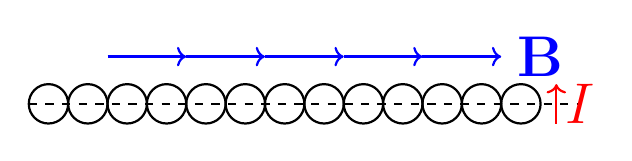
\begin{tikzpicture}

    % Draw solenoid coils
    \foreach \x in {0,0.5,...,6} {
        \draw[thick] (\x,0) arc[start angle=0,end angle=180,radius=0.25];
        \draw[thick] (\x,0) arc[start angle=0,end angle=-180,radius=0.25];
    }

    % Draw the central axis
    \draw[dashed, thick] (-0.5,0) -- (6.5,0);

    % Magnetic field inside solenoid
    \draw[->, blue, thick] (0.5,0.6) -- (1.5,0.6);
    \draw[->, blue, thick] (1.5,0.6) -- (2.5,0.6);
    \draw[->, blue, thick] (2.5,0.6) -- (3.5,0.6);
    \draw[->, blue, thick] (3.5,0.6) -- (4.5,0.6);
    \draw[->, blue, thick] (4.5,0.6) -- (5.5,0.6);
    
    % Label for magnetic field
    \node[blue] at (6,0.6) {\huge $\mathbf{B}$};

    % Current direction (right side)
    \draw[->, red, thick] (6.2,-0.25) -- (6.2,0.25);
    \node[red] at (6.5,0) {\huge $I$};

\end{tikzpicture}
\end{center}
 \end{frame}
 
\begin{frame}
\textcolor{violet}{\textbf{Magnetic field due to torid:}}\\
A toroid is a circular coil with \( N \) turns carrying a current \( I \). We consider an Amperian loop of radius \( r \) inside the toroid along a circular path.

Since the toroid has \( N \) turns, the total enclosed current is:

\begin{equation}
I_{\text{enc}} = N I
\end{equation}

Since the magnetic field inside the toroid is tangential and constant along the loop, the integral simplifies to:


$B (2\pi r) = \mu_0 N I$ On Solving for \( B \):

\[
B = \frac{\mu_0 N I}{2\pi r}
\]


Thus, the magnetic field inside a toroid is:

\[
B = \frac{\mu_0 N I}{2\pi r}
\]

where \( r \) is the radial distance from the center of the toroid. The field is strongest inside the toroid and zero outside.

\end{frame} 


 
\begin{frame}
\textcolor{red}{\textbf{Force between two conductors carrying current:}}\\
\textcolor{violet}{\textbf{When currents are in the same direction:}}\\
Let us conductors A and B in the form of wires placed parallel, r distance away from each other. Let $I_A$ and $I_B$ be the steady currents flowing on wires A and B respectively from bottom to top (i.e.,along same direction).
\begin{center}
\includegraphics[width = 8 cm]{forcingpr}
\end{center}

\end{frame} 
 
 
 \begin{frame}
 \hspace{2cm} $B_A=\frac{\mu_0 I_A}{2\pi r}$ due to $I_A$ is directed to inward,\\
\hspace{2cm} $B_B=\frac{\mu_0 I_B}{2\pi r}$  due to $I_B$ is directed to outward .\\
 Force $F_{BA}$ due to magnetic field $B_A$ is ,\\
 \hspace{1cm} $F_{BA}=B_AI_BL\sin\theta$\\
  where L is segment of wire B for $\theta=90^0$\\
   \hspace{3cm} $F_{BA}=B_AI_BL$\\
  \begin{equation}
  \therefore F_{BA}=\frac{\mu_0 I_A I_B L}{2\pi r}
  \end{equation}
 Similarly, Force $F_{AB}$ due to magnetic field $B_B$ is
 \begin{equation}
 F_{AB}=\frac{\mu_0 I_A I_B L}{2\pi r}
 \end{equation}
 Thus, $F_{AB}=F_{BA}$ The force exerted by the conductors on one another is equal in magnitude and act towards another and force is in attractive nature.
 
 \end{frame}
 

\begin{frame}
\textcolor{violet}{When currents are in opposite direction:}\\
If the direction of the current say $I_A$ is reversed then we see this looks below.
\begin{center}
\includegraphics[width = 5 cm]{dircurd}
\end{center}
The field $B_A$ and $B_B$due to current $I_A, I_B$ is \\

\hspace{3cm} $B_A=\frac{\mu_0 I_A}{2\pi r}$ and $B_B=\frac{\mu_0 I_B}{2\pi r}$ \\
The force experience by each force are same as eariler case but in opposite direction like ,\\
\hspace{2 cm} $F_{AB}=F_{BA}$
This means force are eqaul in magnitude , act away from one another, repulsive in nature.
\end{frame} 
 
 
\begin{frame}
       \textcolor{violet}{\textbf{Hall effect:}}\\
    		\textbf{Definition:} The Hall effect is the production of a voltage difference across an electrical conductor when it is placed in a magnetic field perpendicular to the current flow.  \\
          
       
       \begin{center}
       \includegraphics[width = 6 cm]{halleffect}
       \end{center}
        \begin{itemize}
       \item  \textbf{Voltage Generation} – A voltage is induced perpendicular to both        current and magnetic field.
 \item \textbf{Used in Sensors} – Commonly used in measuring magnetic fields and detecting position or speed.
 \item \textbf{Discovered in 1879} – Found by Edwin Hall, demonstrating charge carrier movement in conductors.
        \end{itemize}
\end{frame}

\begin{frame}
This electric force on the electrons opposes the magnetic force on them and an
equilibrium is reached soon at which these forces balance each other.\\
\[
i.e. F_E=F_B
\]
Let $V_H$ is the potential difference associated with electric field also known as hall voltage ,\\
\[
E=\frac{V_H}{d}
\]
The Electric force $F_E$ experiences by each electron of charge e is ,\\
\[
F_E=eE
\]
Then magnetic force experiences by each electron is \\
\[
BeV_d= eE
\]


\end{frame}


\begin{frame}
\begin{equation}
V_d=\frac{eV_H}{Bed}
\end{equation}

If n be the number of conduction electrons per unit volume of conductor whose crossectional area A then, \\
\hspace{1cm} $V_d=\frac{I}{nAe}$\\
\hspace{3cm}  Finally , $\frac{I}{nAe}=\frac{eV_H}{Bed}$\\
or,$V_H=\frac{BId}{nAe} $ (but $A=d\times t$)\\
\[
V_H=\frac{BI}{net}
\]
we see that hall voltage is inversely proportional to charge density.\\
using $H_c=\frac{1}{ne}$ is hall's coefficiecnt then,\\
\hspace{2cm} $V_H=\frac{BIH_c}{t}$\\
If $R_H$ is the hall resistance $V_H=IR_H \implies R_H=\frac{BH_c}{t}$\\
If J be the current density $J=\frac{I}{A} \implies I=JA $ we get, \\
 
\end{frame}

\begin{frame}
\hspace{1cm} or,  $V_H=\frac{BJAH_c}{t}=BJH_c d$ and$ H_c=(\frac{V_H}{d})\times \frac{1}{BJ}=\frac{E_H}{BJ}$\\
These are the required expression of Hall voltage and hall coeficient by hall effect.\\
\textcolor{blue}{\textbf{Significance of Hall Effect:}}\\
\begin{itemize}
\item[1] Measuring the drift velocity of charge carries:
\item[2] Detecting nature of charge carriers:
\item[3] Hall effect permits the direct measurement of the concentration of the charge carriers (n) in the material.
\end{itemize}

\end{frame}

% Slide for Chapter: Magnetic Properties of Materials
\section{Magnetic Properties of Materials}

\begin{frame}{Magnetic Properties of Materials}
\textcolor{violet}{\textbf{Relative permeability:}}\\
\say{Relative permeability is the ratio of a fluid's effective permeability to the absolute permeability of the porous medium, indicating how easily the fluid flows in the presence of other fluids.}\\

Its denoted by $(\mu_r)$ and given by \\
\[
\mu_r=\frac{\mu}{\mu_0}
\]

And we have this one relation ,\\\  
   \[
   \mu_r=1+\chi
   \]
   where $\chi$ is magnetic susptibility and is defined by \\
   \textcolor{violet}{\textbf{Magnetic suptibility:-}}\\
 \say{Magnetic susceptibility is a measure of how much a material becomes magnetized when exposed to an external magnetic field.} Its denoted by $\chi$  \\
 And the Formula is given  by,\\

\end{frame}


\begin{frame}
 \[
   \chi = \frac{M}{H}
	\]
	Where, \\
	M = magnetization(magnetic moment per unit per unit volume)\\
	H = Applied magnetic field strength.\\
	
\textcolor{violet}{Intensity of Magnetization (M):}\\
\say{It is the magnetic moment per unit volume of a material.}
\[
M=\frac{m}{v}
\]
where m is the magnetic moment and V is the volume\\
\textcolor{violet}{Magneitc Intensity(H):}\\
\say{It is the external magnetic field applied to a material, which induces magnetization.}\\

\[
H=\frac{B}{\mu}-M
\]
where B is the total magnetic field and $\mu$ is permeability.
\end{frame}

\begin{frame}
\textcolor{violet}{Total magnetic field(B):}\\
\say{It is the total magnetic field inside a material, including both external and induced fields.}\\
\[
B=\mu_0(H+M)
\]
where, $\mu_0$ is the permeability in free space.

\textcolor{violet}{\textbf{Relation between Relative permeability and magnetic susptibility:}}\\
As we know definition of permeability for a material medium is givne by \\
\begin{equation}
    \mu = \frac{B}{H}
\end{equation}
Substituting $B$ from Equation TBM;\\
\[
    \mu = \frac{\mu_0 (H + M)}{H}
\]
Dividing by $\mu_0$:
\begin{equation}
    \mu_r = \frac{H + M}{H}
\end{equation}
    
\end{frame}

\begin{frame}


Using Equation From definition of Susptibility;\\
\[
    M = \chi H
\]
Substituting into Equation (21);
\[
    \mu_r = \frac{H + \chi H}{H}
\]
Factoring out $H$:
\begin{equation}
    \mu_r = \frac{H(1 + \chi)}{H}
\end{equation}
Canceling $H$:
\begin{equation}
    \mu_r = 1 + \chi
\end{equation}
This is the required expression of magnetic susptibility and relative permeability.
\end{frame}

\begin{frame}
\textcolor{violet}{Curie Law:}\\
The Curie Law (named after Pierre Curie) describes the magnetic behavior of paramagnetic materials. \\
\textbf{Statemant:} \say{It states that the magnetic susceptibility ($\chi$) of a paramagnetic material is inversely proportional to its absolute temperature (T),}\\
\[
\chi = \frac{C}{T}
\]
where,\\
 $\chi$ Magnetic Susceptibility,\\
C Curie constant\\

T Absolute temperature in (K).\\
\begin{itemize}
\item Temperature of a paramagnetic material increases, its magnetic susceptibility decreases. 
\item At higher temperatures, the random motion of the atoms dominates over the alignment of magnetic moments.
\item  weakening the material's response to an external magnetic field.
\end{itemize}

\end{frame}







\begin{frame}

\textcolor{red}{Understanding Diamagnetic, Paramagnetic, and Ferromagnetic Materials}\\

\textcolor{violet}{\textbf{1. Diamagnetic Materials}}\\
Diamagnetic materials are substances that create an opposing magnetic field when exposed to an external magnetic field. They exhibit a weak negative magnetization.\\

\textbf{Characteristics:}
\begin{itemize}
    \item Weakly repelled by a magnetic field.
    \item Magnetic susceptibility ($\chi$) is \textbf{negative} ($\chi < 0$).
    \item Relative permeability ($\mu_r$) is \textbf{slightly less than 1} ($\mu_r < 1$).
    \item No permanent dipoles; induced dipoles oppose the external field.
    \item Independent of temperature.
\end{itemize}

\textbf{Examples:} Copper (Cu), Gold (Au), Silver (Ag), Lead (Pb), Water, Graphite.

\textcolor{violet}{\textbf{2. Paramagnetic Materials}}\\
Paramagnetic materials are substances that develop a weak magnetization in the direction of an applied magnetic field. Their magnetic effect disappears when the external field is removed.

\end{frame}


\begin{frame}

\textbf{Characteristics:}
\begin{itemize}
    \item Weakly attracted to a magnetic field.
    \item Magnetic susceptibility ($\chi$) is \textbf{positive but small} ($\chi > 0$).
    \item Relative permeability ($\mu_r$) is \textbf{slightly greater than 1} ($\mu_r > 1$).
    \item Presence of unpaired electrons causing small net magnetic moments.
    \item Magnetization follows \textbf{Curie's Law} ($\chi \propto \frac{1}{T}$), meaning it decreases with increasing temperature.
\end{itemize}

\textbf{Examples:} Aluminum (Al), Platinum (Pt), Magnesium (Mg), Oxygen (O$_2$).

\textcolor{violet}{\textbf{3. Ferromagnetic Materials}}\\
Ferromagnetic materials are substances that exhibit strong magnetization in the direction of an applied magnetic field and retain magnetization even after the field is removed (permanent magnetism).

\textbf{Characteristics:}
\begin{itemize}
    \item Strongly attracted to a magnetic field.
    \item Magnetic susceptibility ($\chi$) is \textbf{very large and positive} ($\chi \gg 1$).
    \item Relative permeability ($\mu_r$) is \textbf{much greater than 1} ($\mu_r \gg 1$).
    \item Presence of \textbf{magnetic domains} where atomic dipoles align spontaneously.
    \end{itemize}
\end{frame}



\begin{frame}

\begin{itemize}

\item Retains magnetization even after removing the field (hysteresis effect).
    \item Has a \textbf{Curie temperature} ($T_C$) above which ferromagnetism disappears and behaves as paramagnetic.
\end{itemize}

\textbf{Examples:} Iron (Fe), Cobalt (Co), Nickel (Ni), Steel.

\textcolor{red}{Comparison Table}
\begin{center}
\includegraphics[width= 12 cm]{mtables}
\end{center}

\end{frame}


\begin{frame}
\textcolor{violet}{Hysteresis:}\\
The lag between the applied magnetic field and the material's magnetization, where the material "remembers" past states.\\
\textcolor{violet}{\textbf{Hysteresis loop:}}\\
\say{TA graph showing the relationship between the applied magnetic field (H) and the resulting magnetization (B), demonstrating the material's history-dependent response.}

\begin{center}
\includegraphics[width = 5 cm]{hysteresis}
\end{center}

\end{frame}


\begin{frame}

\begin{itemize}
\item \textcolor{blue}{Coercivity $(H_c)$:} The field strength required to reduce magnetization to zero after full magnetization. High coercivity indicates hard magnets.
\item \textcolor{blue}{Remanence $(B_r)$:} The remaining magnetization when the field is zero. High remanence indicates permanent magnet properties.
\item \textcolor{blue}{Saturation Magnetization (Bs):} The maximum magnetization a material can achieve, beyond which the magnetization does not increase even with a higher field.
\item \textcolor{blue}{Area of the Loop:} Represents energy loss in one cycle of magnetization. Larger area means more energy loss, typical of hard magnetic materials.
\end{itemize}
\textcolor{violet}{Use for Material Types:}\\
\begin{itemize}
\item \textbf{Hard materials:} High coercivity and remanence.
\item \textbf{Soft materials:} Low coercivity and remanence, low energy loss.
\end{itemize}
\end{frame}



% Slide for Chapter: Electromagnetic Induction
\section{Electromagnetic Induction}

\begin{frame}
\textcolor{violet}{Electromagnetic Induction:} \\

Electromagnetic Induction is the process by which a changing magnetic field generates an electric current in a conductor. This phenomenon, discovered by Michael Faraday, forms the basis of many electrical devices, such as generators and transformers. It occurs when a conductor (like a wire) is exposed to a varying magnetic field, causing electrons to move and produce an electric current.\\

\textcolor{blue}{Key: characterostics:}\\

    \begin{itemize}
    \item  Changing Magnetic Field: Induction occurs when the magnetic field around a conductor changes.

\item Induced Current: A changing magnetic field creates an electric current in the conductor.

\item Faraday’s Law: The induced current is proportional to the rate of change of the magnetic field.

\item Lenz’s Law: The induced current opposes the change in the magnetic field.

\item Applications: Used in generators, transformers, and induction motors.
    \end{itemize}
\end{frame}

\begin{frame}
\begin{center}
\includegraphics[width = 10 cm]{magneticfield}
\end{center}
\end{frame}

\begin{frame}
\textcolor{violet}{Magnetic Field:} \say{The region at where the magnetic source modifies the space around it in some manner so that any other magnetic material experience force due to it}\\
\begin{center}
\includegraphics[width =  8 cm]{bdiika}

\end{center}
\textcolor{violet}{Magnetic flux:}\\
Magnetic flux is the total magnetic field passing through a given surface. It is measured in Weber (Wb) and given by $\phi = BA\cos\theta$ where B is the magnetic field, A is the area, and $\theta$ is the angle between them.

\end{frame}

\begin{frame}
\textcolor{violet}{\textbf{Faraday's law of electromagnetic induction:}}\\
\say{Faraday's law states that the induced electromotive force (EMF) in a circuit is directly proportional to the rate of change of magnetic flux through the circuit.}
\begin{itemize}
\item Formula:is magnetic flux. $emf=-\frac{d\phi}{dt}$ where, $\phi$ is magnetic flux.
\item Negative Sign: Indicates Lenz's Law, meaning the induced EMF opposes the change in flux.
\item Faster Change, More EMF: A rapid change in magnetic flux induces a stronger EMF.
\item Practical Applications: Used in transformers, generators, and electric induction devices.
\end{itemize}
\textcolor{violet}{Lenz Law:} \\
\say{Lenz's law states that the direction of the induced current always opposes the change in magnetic flux that caused it.}\\
The induced current has a direction such as to oppose the cause producing it\\
Lenz law is the direct consequence of conservation of energy.
\end{frame}

\begin{frame}
\textcolor{violet}{Lenz law and direction of induced emf}\\
\begin{center}
\includegraphics[width = 10 cm]{direction}
\end{center}
\end{frame}

\begin{frame}
\textcolor{violet}{Construction and working of
A.C. generators}\\
An A.C. generator (alternator) is a device that converts mechanical energy into electrical energy in the form of alternating current (A.C.) based on the principle of electromagnetic induction.\\
\textcolor{blue}{\textbf{Construction:}}
\begin{itemize}
\item Stator: Stationary part with magnetic field.
\item Rotor: Rotating armature coil.
\item Field Magnets: Produce a magnetic field.
\item Slip Rings & Brushes: Transfer A.C. to external circuit.
\end{itemize}
\textcolor{blue}{\textbf{Working:}}
\begin{itemize}
\item The armature coil rotates inside a magnetic field.
\item Due to electromagnetic induction, an A.C. voltage is generated.
\item The slip rings and brushes transfer the alternating current to an external circuit.
\end{itemize}

\end{frame}

\begin{frame}
\item \textbf{Opposition to Change:} Prevents self-sustaining energy generation.
\item \textbf{Energy Input Required:} Work must be done to change flux, converting mechanical to electrical energy.
\item \textbf{No Perpetual Motion:} Stops infinite energy creation, ensuring physics laws hold
\end{itemize}
\textcolor{violet}{Fleming Right Hand Rule}\\
Fleming's Right-Hand Rule:\\
\begin{itemize}

\item Thumb → Motion
\item Index → Field
\item Middle → Current
\end{itemize}
\textcolor{violet}{Eddy Current:}\\
Eddy currents are looping currents induced in conductors when exposed to a changing magnetic field, following Faraday’s Law of electromagnetic induction.
\end{frame}


\begin{frame}
\textcolor{violet}{Self-Inductance (L):}\\
\say{Property of a coil that opposes changes in current by inducing EMF in itself.}
\[
 V_L=-L\frac{dL}{dt}
\]
\textbf{Uses:}
\begin{itemize}
\item Inductors in circuits (filters, oscillators).
\item Chokes (block AC, allow DC).
\item Energy storage in magnetic fields.
\end{itemize}
\textcolor{violet}{Mutual Inductance(M):}\\
\say{Property where a changing current in one coil induces voltage in another coil.}
\[
 V_M=-M\frac{dI}{dt}
\]
\textbf{Uses:}
\begin{itemize}
\item Transformers (power transmission).

\end{itemize}
\end{frame}




\begin{frame}
\begin{itemize}
\item Wireless charging.
\item Coupled circuits (radio, TV tuners).
\end{itemize}
\begin{center}
\includegraphics[width = 4 cm]{inductions}
\end{center}
\end{frame}

\begin{frame}
\textcolor{violet}{\textbf{Energy Stored in an inductor:}}\\
\say{The energy required in the inductor in the form of work done till the current attains a maximum steady value.}\\
As we know the emf related to the self inductance 
\[
E=L\frac{dI}{dt}
\]
If P be the rate at which energy is delivered (power) $P=I.E$
\[
P=L\frac{dI}{dt}.I
\]
Rearranging, $Pdt=L IdI$\\
Integrating from 0 to t and 0 to $I_0$ we get
\[
\int_{0}^{t}Pdt=\int_{0}^{I_0}LIdI
\]

\hspace{1cm} $W=L\int_{0}^{I_0}IdI  \implies W= L[\frac{I}{2}]_{0}^{I_0} \implies W=\frac{1}{2}LI_0^2=U$\\
This is the required expression of energy stored in an inductor.
\end{frame}

\begin{frame}

\textcolor{violet}{\textbf{Emf induced in a rotating coil in uniform magnetic field}}\\
Consider a rectangular coil of surface area A and having N number of turns. The coil is rotated in the uniform magnetic field of \vec{B}. Then magnetic flux linked with coil is ,\\
\[
\phi=NBA\cos\theta
\]
\begin{center}
\includegraphics[width = 7 cm]{rectangularcoil}
\end{center}

\end{frame}


\begin{frame}

Let $\omega$ be the angular velocity of coil then $\theta=\omega t$\\
\hspace{4cm} $\phi=BNA\cos\omega t$\\
Differentiating both side we get,
\[
\frac{d\phi}{dt}=-NBA\omega\sin\omega t
\]
Also we know $E=-\frac{d\phi}{dt}$ we get,
\[
E=-(-NBA\omega \sin\omega t) \implies E=NBA\omega \sin\omega t
\]
The value of induced emf is $E=E_0$ at $\sin\omega t=1$ we get,
 

\[
\therefore E=E_0\sin\omega t
\]

This is the alternating emf (voltage) induced in an inductor. Also E=IR then \\
\[
 I=I_0\sin\omega t
 \]
 This is the alternating current induced in an inductor.
\end{frame}


\begin{frame}
\textcolor{violet}{\textbf{Transformer:}}\\
\say{An electrical device which transforms (changes) an alternating voltage from one value to another of greater or smaller value by using the principle of mutual induction is called transformer.}
\begin{center}
\includegraphics[width = 8 cm]{trnsfermerr}
\end{center}
If $\frac{d\phi}{dt} $ be the rate of flux linked with secondary coil, Then by Faraday law emf ($E_s$) in secondary coil is.
\[
E_s=-N_s\frac{d\phi}{dt}
\]
Here $N_s$ is the turns in the secondary coil. similarly $E_P$ for primary coil is ,
\[
E_p=-N_p\frac{d\phi}{dt}
\]

\end{frame}

\begin{frame}
where $N_P$ is the number of turns in primary coil. Form above this two relations we get,
\[
\frac{E_s}{E_p}=\frac{N_s}{N_p}
\]
This is the known as the transformer equation. \\
If the transformer is $100\%$ efficient , then from energy considerations , \\
\[
V_pI_p=V_s I_s \implies \frac{V_s}{V_p}=\frac{I_p}{I_s}
\]
comparing this with above relation we get,
\[
\frac{N_s}{N_p}=\frac{I_p}{I_s}
\]
\textcolor{violet}{Efficiency of transformer:}\\
\say{The efficiency of transformer is defined as the ratio of output power to input power.}
It is ususally expressed in percentage, So, 
\[
\eta=\frac{I_sV_s}{I_pV_p}\times 100\%
\]

\end{frame}



% Slide for Chapter: Alternating Currents
\section{Alternating Currents}
\begin{frame}{Alternating Currents}
\textcolor{red}{Introduction:}\\
Alternating Current (AC) is an electric current that periodically reverses direction, commonly used in homes and industries. Its ability to be easily transformed makes it ideal for efficient power transmission.
\begin{center}
\includegraphics[width = 8 cm]{accurrent}
\end{center}
\end{frame}

\begin{frame}
\textcolor{violet}{Instantenous value of Ac:}\\
\say{Instantaneous AC refers to the value of alternating current or voltage at any specific moment in time. It varies continuously with the AC waveform. }
instantaneous alternating current is given by,
\[
I(t)=I_0\sin\omega t
\]
where, $I_0$ is the peak value of current.\\
\textcolor{violet}{Peak value of current:}\\
\say{The peak value of alternating quantity is the value of voltage or current at the positive or negative maximum with respect to zero.} This is also called as amplitudes of alternating quantity $I_0$.
\begin{center}
\includegraphics[width = 9 cm]{peakvalueac}
\end{center}

\end{frame}

\begin{frame}
\textcolor{violet}{Average or mean value of A.C}\\
\say{The average (mean) value of AC over a full cycle is zero because the positive and negative halves cancel out. However, over a half-cycle, it is given by:}
\[
i.e\hspace{1cm} I_{av}=\frac{2}{\pi}I_0 \hspace{1cm} or, \hspace{1cm} V_{av}=\frac{2}{\pi}V_0
\]
Where, $I_0$ and $V_0$ are the maximum value of current and voltage.\\

\textcolor{violet}{Proof:}\\

The average value of an alternating current (AC) or voltage is calculated over a half-cycle, as the full-cycle average is zero due to symmetry.

For a sinusoidal AC voltage or current:

\[
V = V_0 \sin\theta
\]

where \( V_0 \) is the peak value and \( \theta \) is the phase angle (in radians).

\textbf{Step 1: Formula for Average Value}
The average value over a half-cycle (0 to \( \pi \)) is given by:

\end{frame}

\begin{frame}

\[
V_{\text{avg}} = \frac{1}{\pi} \int_0^\pi V_0 \sin\theta \, d\theta
\]

\textbf{Step 2: Evaluating the Integral}

\[
V_{\text{avg}} = \frac{V_0}{\pi} \int_0^\pi \sin\theta \, d\theta
\]

We know that: \textcolor{blue}{$\int \sin\theta \, d\theta = -\cos\theta$}\\


Applying limits from \( 0 \) to \( \pi \):

\[
\left[-\cos\theta\right]_0^\pi = -\cos\pi + \cos 0 = -(-1) + 1 = 1 + 1 = 2
\]

\textbf{Step 3: Final Expression}

\[
V_{\text{avg}} = \frac{V_0}{\pi} \times 2 = \frac{2V_0}{\pi}
\]

Thus, the \textbf{average or mean value of AC} over a half-cycle is:

\[
V_{\text{avg}} = \frac{2V_0}{\pi} \hspace{1cm} or \hspace{1cm} I_{\text{avg}} = \frac{2I_0}{\pi}
\]

\end{frame}

\begin{frame}
\textcolor{violet}{\textbf{RMS value of AC}}\\
The RMS value of an alternating current (AC) or voltage is the effective value that produces the same heating effect as a direct current (DC) of the same magnitude. It is mathematically defined as:
\[
V_{rms}=\sqrt{\frac{1}{T}\int_{0}^{T}v^2dt}
\]
For Sinusoidal AC voltage or current:
\[
V=V_0\sin\theta
\]
The RMS value over one full cycle is defined as:
\[
V_{rms}=\frac{V_0}{\sqrt{2}}
\]
Similarly, For current: 
\[
 I_{rms}=\frac{I_0}{\sqrt{2}}
 \]
 The RMS value is widely used in electrical calculations, as it represents the practical or effective value of AC in power systems.
\end{frame}


\begin{frame}
\textcolor{blue}{Proof For $I_{rms}$ value of AC}\\
The RMS value of AC current over one full cycle is given by:

\[
I_{\text{rms}} = \sqrt{\frac{1}{T} \int_0^T I^2 dt}
\]

For a sinusoidal AC current: $I = I_0 \sin\theta$

where \( I_0 \) is the peak current , And the RMS formula becomes:

\[
I_{\text{rms}} = \sqrt{\frac{1}{2\pi} \int_0^{2\pi} I_0^2 \sin^2\theta \, d\theta}
\]

Using the standard integral identity: $\int_0^{2\pi} \sin^2\theta \, d\theta = \frac{2\pi}{2} = \pi$\\

\[
I_{\text{rms}} = \sqrt{\frac{I_m^2}{2\pi} \times \pi}
\]
$I_{\text{rms}} = \sqrt{\frac{I_0^2}{2}} \implies I_{\text{rms}} = \frac{I_0}{\sqrt{2}} $ 



RMS value of a sinusoidal AC waveform is \(\frac{1}{\sqrt{2}}\) times its peak value.

\end{frame}

\begin{frame}
\textcolor{violet}{\textbf{Phasors:}}\\
\say{Phasors are complex numbers representing sinusoidal signals, showing both magnitude and phase.} Phasor representation is used to study the phase relationship between two sinusoidally varying quantities having same frequency.
\begin{center}
\includegraphics[width = 10 cm]{phasors}
\end{center}
\end{frame}


\begin{frame}
\textcolor{violet}{Phase shift between two wave forms:}\\
The phase shift between two waveforms is the difference in their phase angles, 
\[
\Delta\theta=\theta_2-\theta_1
\]

\textcolor{blue}{Interpretation:}
\begin{itemize}
\item Positive $\Delta\theta$→ Waveform 2 leads Waveform 1.
\item Negative $\Delta\theta$ → Waveform 2 lags Waveform 1.
\item $180^0$ phase shift → The waveforms are completely out of phase.
\item $0^0$ or $360^0$ phase shift → The waveforms are in phase (aligned).
\end{itemize} 
If the waveforms have the same frequency f, the phase shift can also be expressed in time t as:
\[
\Delta t=\frac{\Delta\theta}{360^0}\times T
\]

\end{frame}

\begin{frame}
\textcolor{violet}{\textbf{A.C. Through Resistor:}}\\
\includegraphics[width = 6 cm]{giftforgf}
\includegraphics[width = 5 cm]{phasorofres}\\
\textbf{Apply Kirchhoff’s Voltage Law (KVL)}


For a purely resistive circuit with an applied AC voltage:

\[
V(t) = V_0 \sin(\omega t)
\]

where: \( V_0 \) = peak voltage  \( \omega = 2\pi f \) = angular frequency  
    and \( t \) = time  \\

Using \textbf{Ohm’s Law}: $I(t) = \frac{V(t)}{R}$

\hspace{6cm} $I(t) = \frac{V_0\sin(\omega t)}{R}$\\
Define peak current as:  $I_0 = \frac{V_0}{R}$
Thus, the equation simplifies to:

\[
I(t) = I_0 \sin(\omega t)
\]

Thus: The current \( I(t) \) is a sinusoidal function with the same frequency \( \omega \) as the voltage, proving that the current through a resistor is sinusoidal.
\end{frame}

\begin{frame}
\textcolor{violet}{\textbf{A.C. Through Inductor:}}\\

\includegraphics[width = 5 cm]{acthroughind}
\includegraphics[width = 5 cm]{phasoroflc}\\
\textbf{Apply Kirchhoff’s Voltage Law (KVL)}

For an inductor \( L \) in an AC circuit, the applied voltage is:

\[
V(t) = V_0 \sin(\omega t)
\]

Using the inductor voltage-current relationship:

\[
V(t) = L \frac{dI(t)}{dt}
\]

\textbf{Step 2: Solve for \( I(t) \)}

\[
L \frac{dI(t)}{dt} = V_0 \sin(\omega t)
\]
\end{frame}



\begin{frame}

Dividing both sides by \( L \):

\[
\frac{dI(t)}{dt} = \frac{V_0}{L} \sin(\omega t)
\]

Integrating both sides:

\[
I(t) = \int \frac{V_0}{L} \sin(\omega t) dt
\]

\[
I(t) = \frac{V_0}{L} \int \sin(\omega t) dt
\]

Using the integral:

\[
\int \sin(\omega t) dt = -\frac{\cos(\omega t)}{\omega}
\]

\[
I(t) = -\frac{V_0}{L \omega} \cos(\omega t)
\]

Since \( \cos(\omega t) = \sin(\omega t + 90^\circ) \), we rewrite:

\end{frame}

\begin{frame}


\[
I(t) = I_0 \sin(\omega t - 90^\circ)
\]

where:

\[
I_0 = \frac{V_0}{\omega L}
\]

\textbf{Step 3: Phase Relationship}

\begin{itemize}
    \item The current \textbf{lags} the voltage by \textbf{90°} (or \( \frac{\pi}{2} \) radians).
    \item The inductor \textbf{opposes} changes in current, causing a \textbf{phase shift}.
\end{itemize}

\textbf{Conclusion}

For AC through an inductor: $I(t) = I_0 \sin(\omega t - 90^\circ)$

\begin{itemize}
    \item The current \textbf{lags} voltage by \textbf{90°}.
    \item The inductive \textbf{reactance} is given by \( X_L = \omega L \), where \( \omega = 2\pi f \).
    \item The peak current is \( I_0 = \frac{V_0}{X_L} \).
		\end{itemize}

\end{frame}

\begin{frame}
\textcolor{violet}{\textbf{A.C. Through Capacitor:}}\\
\includegraphics[width = 6 cm]{capacatorsac}
\includegraphics[width = 5 cm]{phasorofcapa}\\

\textbf{Apply Kirchhoff’s Voltage Law (KVL)}

For a capacitor \( C \) in an AC circuit, the applied voltage is:

\[
V(t) = V_0 \sin(\omega t)
\]

Using the capacitor voltage-current relationship:

\[
I(t) = C \frac{dV(t)}{dt}
\]

\textbf{Solve for \( I(t) \)} \hspace{2cm} $I(t) = C \frac{d}{dt} \left( V_0 \sin(\omega t) \right)$



\end{frame}


\begin{frame}

Taking the derivative:

\[
I(t) = C V_0 \omega \cos(\omega t)
\]

Since \( \cos(\omega t) = \sin(\omega t + 90^\circ) \), we rewrite:

\[
I(t) = I_0 \sin(\omega t + 90^\circ)
\]

where:

\[
I_0 = V_0 \omega C
\]

\textbf{Phase Relationship}

\begin{itemize}
    \item The current \textbf{leads} the voltage by \textbf{90°} (or \( \frac{\pi}{2} \) radians).
    \item The capacitor \textbf{opposes} changes in voltage, causing a \textbf{phase shift}.
\end{itemize}

\textbf{Capacitive Reactance}

The capacitive reactance \( X_C \) is given by:

\[
X_C = \frac{1}{\omega C}
\]
\end{frame}


\begin{frame}
Thus, the peak current can be written as:

\[
I_0 = \frac{V_0}{X_C}
\]

\textbf{Conclusion}

For AC through a capacitor:

\[
I(t) = I_0 \sin(\omega t + 90^\circ)
\]

\begin{itemize}
    \item The current \textbf{leads} voltage by \textbf{90°}.
    \item The capacitive \textbf{reactance} is given by \( X_C = \frac{1}{\omega C} \).
    \item The peak current is \( I_0 = \frac{V_0}{X_C} \).
\end{itemize}
\end{frame}


\begin{frame}
\textcolor{violet}{\textbf{A.C. Through R–L Series Circuit:}}\\
\begin{center}
\includegraphics[width = 6 cm]{Acthroughrl}
\end{center}
\textbf{Apply Kirchhoff’s Voltage Law (KVL)}

Consider an R-L series circuit with an applied voltage \( V(t) = V_0 \sin(\omega t) \). The total voltage across the resistor and inductor is:

\[
V(t) = V_R(t) + V_L(t)
\]

Using Ohm's Law for the resistor:

\[
V_R(t) = I(t) R
\]

And for the inductor:

\[
V_L(t) = L \frac{dI(t)}{dt}
\]

Thus, applying Kirchhoff’s Voltage Law (KVL):

\end{frame}

\begin{frame}

\[
V_0 \sin(\omega t) = I(t) R + L \frac{dI(t)}{dt}
\]

\textbf{Solve the Differential Equation}

This is a first-order linear differential equation:

\[
L \frac{dI(t)}{dt} + I(t) R = V_0 \sin(\omega t)
\]

Solve the homogeneous equation first:

\[
L \frac{dI_h(t)}{dt} + I_h(t) R = 0
\]

The solution to the homogeneous equation is:

\[
I_h(t) = A e^{-\frac{R}{L} t}
\]

Next, solve the non-homogeneous equation using the method of undetermined coefficients. Assume a solution of the form:

\[
I(t) = I_0 \sin(\omega t + \phi)
\]

\end{frame}
\begin{frame}

Substitute this into the equation \( L \frac{dI(t)}{dt} + I(t) R = V_0 \sin(\omega t) \):

\[
L \cdot I_0 \omega \cos(\omega t + \phi) + I_0 R \sin(\omega t + \phi) = V_0 \sin(\omega t)
\]

Using trigonometric identities, we get:

\[
I_0 (L \omega \cos(\omega t + \phi) + R \sin(\omega t + \phi)) = V_0 \sin(\omega t)
\]

Equating the coefficients of \( \sin(\omega t) \) and \( \cos(\omega t) \), we get two equations:

\[
I_0 R \cos(\phi) = V_0 \quad \text{(coefficient of } \sin(\omega t))
\]

\[
I_0 L \omega \sin(\phi) = 0 \quad \text{(coefficient of } \cos(\omega t))
\]

\textbf{Solve for \( I_0 \) and \( \phi \)}

From the first equation:

\[
I_0 = \frac{V_0}{\sqrt{R^2 + (L \omega)^2}}
\]

From the second equation, solving for the phase angle \( \phi \):

\end{frame}

\begin{frame}


\[
\tan(\phi) = \frac{L \omega}{R}
\]

Thus, the phase angle \( \phi \) is:

\[
\phi = \tan^{-1}\left(\frac{L \omega}{R}\right)
\]

\textbf{Current Expression}

The current in the circuit is:

\[
I(t) = I_0 \sin(\omega t + \phi)
\]

where:

\[
I_0 = \frac{V_0}{\sqrt{R^2 + (L \omega)^2}}, \quad \phi = \tan^{-1}\left(\frac{L \omega}{R}\right)
\]

\textbf{Conclusion}

For an R-L series circuit, the current \( I(t) \) is sinusoidal with:

\end{frame}

\begin{frame}

\begin{itemize}
    \item The peak current \( I_0 = \frac{V_0}{\sqrt{R^2 + (L \omega)^2}} \).
    \item The phase shift \( \phi = \tan^{-1}\left(\frac{L \omega}{R}\right) \), indicating that the current \textbf{lags} the voltage by a phase angle \( \phi \).
\end{itemize}

\textbf{Impedance of R-L Circuit}

The total impedance \( Z \) of the R-L circuit is:

\[
Z = \sqrt{R^2 + (L \omega)^2}
\]

Thus, the peak current can be expressed as:

\[
I_0 = \frac{V_0}{Z}
\]

\end{frame}



\begin{frame}
\textcolor{violet}{\textbf{A.C. Through R-C Circuit:}}
\begin{center}
\includegraphics[width = 8 cm]{acthroughrc}
\end{center}
\textbf{Apply Kirchhoff’s Voltage Law (KVL)}

Consider an R-C series circuit with an applied AC voltage \( V(t) = V_0 \sin(\omega t) \). The total voltage across the resistor and capacitor is:

\[
V(t) = V_R(t) + V_C(t)
\]

Using Ohm’s Law for the resistor:

\[
V_R(t) = I(t) R
\]

For the capacitor, the voltage is related to the current by:

\[
V_C(t) = \frac{1}{C} \int I(t) dt
\]

\end{frame}

\begin{frame}

Thus, applying Kirchhoff’s Voltage Law:

\[
V_0 \sin(\omega t) = I(t) R + \frac{1}{C} \int I(t) dt
\]

\textbf{Solve the Differential Equation}

Taking the derivative of both sides of the equation with respect to time:

\[
\frac{d}{dt} \left( V_0 \sin(\omega t) \right) = R \frac{dI(t)}{dt} + \frac{I(t)}{C}
\]

Simplifying:

\[
V_0 \omega \cos(\omega t) = R \frac{dI(t)}{dt} + \frac{I(t)}{C}
\]

This is a first-order linear differential equation. To solve it, we use the method of undetermined coefficients, assuming a solution of the form:

\[
I(t) = I_0 \sin(\omega t + \phi)
\]

\textbf{Substitute the Assumed Solution}

\end{frame}

\begin{frame}

Substitute \( I(t) = I_0 \sin(\omega t + \phi) \) into the differential equation. First, calculate the derivative:

\[
\frac{dI(t)}{dt} = I_0 \omega \cos(\omega t + \phi)
\]

Substitute into the equation:

\[
V_0 \omega \cos(\omega t) = R I_0 \omega \cos(\omega t + \phi) + \frac{I_0 \sin(\omega t + \phi)}{C}
\]

Using trigonometric identities, we get:

\[
I_0 \left( R \omega \cos(\omega t + \phi) + \frac{\sin(\omega t + \phi)}{C} \right) = V_0 \omega \cos(\omega t)
\]

\textbf{Solve for the Amplitude and Phase Shift}

By equating the coefficients of \( \sin(\omega t) \) and \( \cos(\omega t) \), we get:

\[
I_0 \left( R \omega \cos(\phi) + \frac{1}{C} \sin(\phi) \right) = V_0 \omega
\]

From this, the magnitude of the current is:


\end{frame}


\begin{frame}


\[
I_0 = \frac{V_0}{\sqrt{R^2 + \left( \frac{1}{C \omega} \right)^2}}
\]

The phase angle \( \phi \) is given by:

\[
\tan(\phi) = \frac{\frac{1}{C \omega}}{R}
\]

Thus, the phase shift \( \phi \) is:

\[
\phi = \tan^{-1}\left( \frac{1}{R C \omega} \right)
\]

\textbf{Current Expression}

Finally, the current in the circuit is:

\[
I(t) = I_0 \sin(\omega t + \phi)
\]

where:
\end{frame}


\begin{frame}

\[
I_0 = \frac{V_0}{\sqrt{R^2 + \left( \frac{1}{C \omega} \right)^2}}, \quad \phi = \tan^{-1}\left( \frac{1}{R C \omega} \right)
\]

\textbf{Conclusion}

For an R-C series circuit, the current \( I(t) \) is sinusoidal with:

\begin{itemize}
    \item The peak current \( I_0 = \frac{V_0}{\sqrt{R^2 + \left( \frac{1}{C \omega} \right)^2}} \).
    \item The phase shift \( \phi = \tan^{-1}\left( \frac{1}{R C \omega} \right) \), indicating that the current \textbf{lags} the voltage.
\end{itemize}

The \textbf{impedance} \( Z \) of the circuit is:

\[
Z = \sqrt{R^2 + \left( \frac{1}{C \omega} \right)^2}
\]

The peak current can also be written as:

\[
I_0 = \frac{V_0}{Z}
\]

\end{frame}

\begin{frame}
\textcolor{violet}{\textbf{L-C-R Series Circuit in A.C:}}
\begin{center}
\includegraphics[width = 7 cm]{lcrfromc}
\end{center}
Apply Kirchhoff’s Voltage Law (KVL),
Consider an L-C-R series circuit with an applied AC voltage \( V(t) = V_0 \sin(\omega t) \). The total voltage across the resistor, inductor, and capacitor is:

\[
V(t) = V_R(t) + V_L(t) + V_C(t)
\]

Using Ohm’s Law for the resistor:

V_R(t) = I(t) R


For the inductor:

\[
V_L(t) = L \frac{dI(t)}{dt}
\]


\end{frame}



\begin{frame}
For the capacitor:

\[
V_C(t) = \frac{1}{C} \int I(t) dt
\]

Thus, applying Kirchhoff’s Voltage Law:

\[
V_0 \sin(\omega t) = I(t) R + L \frac{dI(t)}{dt} + \frac{1}{C} \int I(t) dt
\]

Take the derivative of both sides with respect to time:

\[
\frac{d}{dt} \left( V_0 \sin(\omega t) \right) = R \frac{dI(t)}{dt} + L \frac{d^2I(t)}{dt^2} + \frac{I(t)}{C}
\]

Simplifying:

\[
V_0 \omega \cos(\omega t) = R \frac{dI(t)}{dt} + L \frac{d^2I(t)}{dt^2} + \frac{I(t)}{C}
\]

This is a second-order linear differential equation. To solve it, we assume a solution of the form:

\end{frame}



\begin{frame}

\[
I(t) = I_0 \sin(\omega t + \phi)
\]

Substitute \( I(t) = I_0 \sin(\omega t + \phi) \) into the differential equation. First, compute the derivatives:

\[
\frac{dI(t)}{dt} = I_0 \omega \cos(\omega t + \phi)
\]

\[
\frac{d^2I(t)}{dt^2} = -I_0 \omega^2 \sin(\omega t + \phi)
\]

Substitute these into the equation:

\[
V_0 \omega \cos(\omega t) = R I_0 \omega \cos(\omega t + \phi) + L (-I_0 \omega^2 \sin(\omega t + \phi)) + \frac{I_0 \sin(\omega t + \phi)}{C}
\]

Using trigonometric identities, we get:



$I_0 \left( R \omega \cos(\omega t + \phi) + \frac{\sin(\omega t + \phi)}{C} - L \omega^2 \sin(\omega t + \phi) \right) = V_0 \omega \cos(\omega t)$
\end{frame}


\begin{frame}

\textcolor{violet}{\textbf{Amplitude and Phase Shift}}

By equating the coefficients of \( \sin(\omega t) \) and \( \cos(\omega t) \), we obtain:

\begin{itemize}
    \item Coefficients of \( \cos(\omega t) \):
    \[
    I_0 \omega \left( R \cos(\phi) - L \omega \sin(\phi) \right) = V_0 \omega
    \]

    \item Coefficients of \( \sin(\omega t) \):
    \[
    I_0 \omega \left( R \sin(\phi) + L \omega \cos(\phi) \right) = 0
    \]
\end{itemize}

Solve these two equations for the amplitude \( I_0 \) and phase \( \phi \).

The amplitude of the current is:

\[
I_0 = \frac{V_0}{\sqrt{R^2 + \left( L \omega - \frac{1}{C \omega} \right)^2}}
\]

The phase shift \( \phi \) is given by:


\hspace{3cm}$\tan(\phi) = \frac{L \omega - \frac{1}{C \omega}}{R}$

Thus, the phase shift \( \phi \) is:
\end{frame}


\begin{frame}

\[
\phi = \tan^{-1}\left( \frac{L \omega - \frac{1}{C \omega}}{R} \right)
\]

Finally, the current in the circuit is:

\[
I(t) = I_0 \sin(\omega t + \phi)
\]

where:

\[
I_0 = \frac{V_0}{\sqrt{R^2 + \left( L \omega - \frac{1}{C \omega} \right)^2}}, \quad \phi = \tan^{-1}\left( \frac{L \omega - \frac{1}{C \omega}}{R} \right)
\]

The total impedance \( Z \) of the L-C-R circuit is:

\[
Z = \sqrt{R^2 + \left( L \omega - \frac{1}{C \omega} \right)^2}
\]
\end{frame}


\begin{frame}

Thus, the peak current can also be written as:

\[
I_0 = \frac{V_0}{Z}
\]

\textbf{Conclusion}

For an L-C-R series circuit, the current \( I(t) \) is sinusoidal with:

\begin{itemize}
    \item The peak current \( I_0 = \frac{V_0}{\sqrt{R^2 + \left( L \omega - \frac{1}{C \omega} \right)^2}} \).
    \item The phase shift \( \phi = \tan^{-1}\left( \frac{L \omega - \frac{1}{C \omega}}{R} \right) \), indicating that the current may \textbf{lead or lag} the voltage depending on the relative values of \( L \), \( C \), and \( R \).
\end{itemize}

The impedance of the circuit is:

\[
Z = \sqrt{R^2 + \left( L \omega - \frac{1}{C \omega} \right)^2}
\]

\end{frame}


\begin{frame}



Where:
\begin{itemize}
    \item \( R \) is the resistance,
    \item \( L \) is the inductance,
    \item \( C \) is the capacitance,
    \item \( \omega \) is the angular frequency of the AC source.
\end{itemize}

\textbf{Condition for Resonance}

Resonance occurs when the reactive component (inductive reactance \( X_L = L \omega \) and capacitive reactance \( X_C = \frac{1}{C \omega} \)) cancel each other out. This happens when:

\[
X_L = X_C \quad \Rightarrow \quad L \omega = \frac{1}{C \omega}
\]

\textbf{for Angular Frequency}

From the condition \( L \omega = \frac{1}{C \omega} \), we solve for \( \omega \):

\[
L \omega^2 = \frac{1}{C} \quad \Rightarrow \quad \omega^2 = \frac{1}{LC}
\]
\end{frame}


\begin{frame}

Thus, the angular frequency at resonance is:

\[
\omega_0 = \frac{1}{\sqrt{LC}}
\]

\textbf{Resonance Frequency}

The resonance frequency \( f_0 \) in Hertz is related to the angular frequency \( \omega_0 \) by:

\[
f_0 = \frac{\omega_0}{2 \pi} = \frac{1}{2 \pi \sqrt{LC}}
\]
\textcolor{blue}{Three special Cases:}

\textbf{1. Inductive Case (When the circuit is inductive)}

\textbf{Condition}: \( X_L > X_C \) (Inductive reactance greater than capacitive reactance)

\[
Z = \sqrt{R^2 + \left( X_L - X_C \right)^2}
\]
Where \( X_L = L \omega \) and \( X_C = \frac{1}{C \omega} \).

\textbf{Phase}: The current \textit{lags} the voltage by an angle \( \phi \) where:
\end{frame}


\begin{frame}

\[
\tan(\phi) = \frac{X_L - X_C}{R}
\]

\textbf{2. Capacitive Case (When the circuit is capacitive)}

\textbf{Condition}: \( X_L < X_C \) (Capacitive reactance greater than inductive reactance)

\[
Z = \sqrt{R^2 + \left( X_C - X_L \right)^2}
\]
Where \( X_L = L \omega \) and \( X_C = \frac{1}{C \omega} \).

\textbf{Phase}: The current \textit{leads} the voltage by an angle \( \phi \) where:
\[
\tan(\phi) = \frac{X_C - X_L}{R}
\]

\textbf{3. Resonance Case (When the circuit is at resonance)}

\textbf{Condition}: \( X_L = X_C \) (Inductive reactance equals capacitive reactance)
\[
L \omega = \frac{1}{C \omega}
\]
\end{frame}


\begin{frame}
\textbf{Impedance}: 
\[
Z = R
\]
The impedance is minimized, and the current is maximized.

\textbf{Phase}: The current and voltage are \textit{in phase} (i.e., \( \phi = 0 \)).
\begin{center}
\includegraphics[width = 8 cm]{gdgG}
\end{center}

\end{frame}

\begin{frame}
\textcolor{violet}{\textbf{Power in LCR Circuit:}}\\
\textbf{Voltage and Current in an LCR Circuit}

For an AC voltage source:
\[
    V = V_0 \cos(\omega t)
    \]

Let the current through the circuit be:
\[
    I = I_0 \cos(\omega t - \phi)
\]
where:
\begin{itemize}
    \item $V_0$ and $I_0$ are the peak voltage and peak current,
    \item $\omega$ is the angular frequency,
    \item $\phi$ is the phase angle between voltage and current.
\end{itemize}
\[
    Z = \sqrt{R^2 + (X_L - X_C)^2}
\]
   \hspace{2cm} $X_L &= \omega L \quad \text{(Inductive Reactance)}$ \\
    \hspace{2cm} $X_C &= \frac{1}{\omega C} \quad \text{(Capacitive Reactance)}$
    \end{frame}
   
   
    \begin{frame}
The phase angle is given by:
\[
    \tan \phi = \frac{X_L - X_C}{R}
\]

\textbf{Instantaneous Power} $  P(t) = V(t) \cdot I(t)$
Substituting the values of $V$ and $I$:
\[
    P(t) = V_0 \cos(\omega t) \cdot I_0 \cos(\omega t - \phi)
\]
Using the trigonometric identity:
\[
    \cos A \cos B = \frac{1}{2} [\cos(A - B) + \cos(A + B)]
\]
we get:
\[
    P(t) = \frac{V_0 I_0}{2} [\cos \phi + \cos(2\omega t - \phi)]
\]

\textbf{Average Power (Real Power)}
The average power over a complete cycle is given by:
\[
    P_{\text{avg}} = \frac{1}{T} \int_0^T P(t) dt
\]
Since the integral of $\cos(2\omega t - \phi)$ over one cycle is zero, we obtain:

\end{frame}


\begin{frame}
\[
    P_{\text{avg}} = \frac{V_0 I_0}{2} \cos \phi
\]

Using RMS values ($V_{\text{rms}} = \frac{V_0}{\sqrt{2}}$ and $I_{\text{rms}} = \frac{I_0}{\sqrt{2}}$), we rewrite the expression as:
\[
    P_{\text{avg}} = V_{\text{rms}} I_{\text{rms}} \cos \phi
\]
$P_{\text{avg}} = V_{\text{rms}} I_{\text{rms}} \cos \phi$, which determines the actual energy consumed in the circuit.\\
 
\textcolor{violet}{Q Factor in LCR Circuit}\\
The Q Factor (Quality Factor) of an LCR circuit is a dimensionless parameter that measures the sharpness of resonance in the circuit.\\
 It is defined as:
\[
Q=\frac{Resonant \ Frequency (f_0)}{Bnadwidth(\Delta f)}
\]
Equivalently, 
\[
Q=\frac{\omega_0 L}{R}=\frac{1}{R}\sqrt{\frac{L}{C}}
\]

\end{frame}

\begin{frame}

Where: $f_0= \frac{1}{2\pi}\sqrt{\frac{1}{LC}}$ is resonant frequency, $\Delta f=\frac{R}{2\pi L} $ is Bandwidth\\
$\omega_0=2\pi f_0$ is angular resonant frequency, R,L,C have their usual meaning.
\vspace{1cm}

\end{frame}

\begin{frame}
\section*{Acknowledgement}
\begin{center}
\textcolor{myNewColorC}{\Huge{\centerline{Thank you!}}}
\end{center}

\end{frame}

\section*{Reference}  
\begin{frame}{Reference}
\scriptsize
\bibliographystyle{apalike}
\bibliography{ref}
\begin{itemize}
\item[1]\textbf{R. Pd.Koirala ,PRINCIPLES OF
PHYSI CS - II, Asmita Books Publishers and Distributors (P) Ltd.}
\item[2] \textbf{https://www.deepseek.com and https://openai.com/index/chatgpt/}

\end{itemize}
\end{frame}





\end{document}
